\documentclass[output=paper]{langsci/langscibook}
\ChapterDOI{10.5281/zenodo.4280645}

\author{Howard Lasnik\affiliation{University of Maryland at College Park}\lastand Zach Stone\affiliation{University of Maryland at College Park}}
\title{Rethinking phrase structure}

% \chapterDOI{} %will be filled in at production

\abstract{We investigate structural properties of two set-theoretic models of
    \isi{phrase structure}, namely the phrase markers of LSLT and bare phrase
    structure. We demonstrate that neither set-theoretic model has a nice
    notion of “substructure” which is well-behaved with respect to the
extension condition. We compare these with graph- and order-theoretic
representations which have well-behaved structure-preserving maps for
characterizing both the extension condition and the operation \isi{Agree}.}

\maketitle

\begin{document}\glsresetall

\section{Introduction}

We review two models of \isi{phrase structure} in Generative Grammar and survey their
structural properties with respect to substructures and isomorphism\is{isomorphism}. We
especially look at how these structural notions bear on the extension
condition. Specifically, we show that neither formal representation captures a
sufficiently general form of the extension condition, while the correct
properties are captured straightforwardly both by graph- and order-theoretic
representations.

We use standard set-theoretic notation: we sometimes indicate a set by writing
its elements  in braces $A=\{a_i\}_{i\in I}$; we use the symbol $A\subset B$ to
represent that every element of $A$ is an element of $B$, called a (potentially
improper) subset; we use $A\cong B$ to indicate that there is some bijection
between the sets; we use $A\cup B$ to represent the union of two sets; we use
$A^*$ to represent the set of all \emph{words}, or strings of finite length
spelled from symbols of $A$; we represent a set-function $f:A\rightarrow B$, or
sometimes just $A\rightarrow B$.

We discuss substructures and isomorphism\is{isomorphism} somewhat informally, though all forms
of them discussed can be made precise in the language of model theory or
category theory.

\section{Phrase markers and reduced phrase markers}

\citet{conceptions} briefly points out an issue that arises with respect to the
\gls{EC}, the Minimalist version of the principle of the cycle proposed by
\citet{Chomsky1993}, or, more precisely, the deduction of it by
\citet{Chomsky2000}. \textcite[22]{Chomsky1993} formulated \gls{EC}\is{extension
condition} as follows:

\ea\label{ex:33.1} GT [generalized
    transformation] and Move $\alpha$ extend K to K$'$ which includes K
    as a proper part.
\z

The \textcite{Chomsky2000} rationale for \gls{EC}\is{extension condition} is that derivations conform to a
condition demanding that there be no tampering by a transformation with already
existing structure. If an item is newly attached at the \enquote{top} of a tree, the
former tree is assumed to be completely preserved as a sub-tree by external
merge, and also by internal merge\is{Merge} on the \isi{copy theory of
movement}. Here's a
simplified toy illustration. Start with the tree in \eqref{ex:33.2}.

\begin{multicols}{2}
\ea\label{ex:33.2}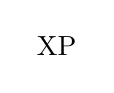
\begin{tikzpicture}[baseline=(root.base)]
        \Tree [.\node(root){XP}; [.X ] [.YP [.Y ] [.ZP [.Z ] ] ] ]
    \end{tikzpicture}
\ex\label{ex:33.3}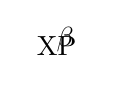
\begin{tikzpicture}[baseline=(root.base)]
    \Tree [.\node(root){XP}; [.$\beta$ ] [.XP [.X ] [.YP [.Y ] [.ZP [.Z ] ] ] ] ]
\end{tikzpicture}
\z
\end{multicols}

Now suppose $\beta$ is adjoined\is{adjunction} to XP in accord with
\eqref{ex:33.1}. The resulting tree is \eqref{ex:33.3}, which clearly
includes \eqref{ex:33.2} as a sub-tree, the intended consequence.

But now consider these structures in terms of their set-theoretic
representations, for example, as in LSLT \parencite{Chomsky1955}. The picture
in \eqref{ex:33.2} stands for the actual object in \eqref{ex:33.4}, a
set of strings:\largerpage

\ea\label{ex:33.4}$\{\text{XP, X YP, X Y ZP, X Y Z}\}$
\z

\noindent And the picture in \eqref{ex:33.3} stands for the actual derived object in
\eqref{ex:33.5}:

\ea\label{ex:33.5}\{\text{XP, $\beta$ XP, $\beta$ X YP, $\beta$ X Y ZP, $\beta$ X Y Z}\}
\z

Notice that \eqref{ex:33.4} is in no respect a sub-object, i.e., a subset, of \eqref{ex:33.5}. And this
is not because of any special property of the example chosen. It is invariably
true that if we adjoin something to the \enquote{top} of an
LSLT-style \gls{PM}\is{phrase marker}, the resulting set is never a superset
of the original. That is, we have dramatically \enquote{tampered} with the original
set: It is gone.

It is important to realize that the same conclusion follows on any \enquote{purely} set
theoretic implementation of syntactic theory. One other such implementation is
that of \citet{lk}. In that framework as in that of LSLT, a
\gls{PM} is a set of strings. The difference is that for L\&K the \gls{PM}\is{phrase marker} consists
entirely of the terminal string and \enquote{monostrings} (strings comprised of exactly
one non-terminal symbol surrounded by any number of terminal symbols). L\&K
called their \glspl{PM} \glspl{RPM}. To see that the same conclusion outlined
above happens with \glspl{RPM}, we need to slightly complicate the example
discussed, since there, it turns out that the \gls{PM}\is{phrase marker} and \gls{RPM}\is{reduced phrase marker} are the
same. So consider the slightly more complex tree in \eqref{ex:33.6}:

\ea\label{ex:33.6}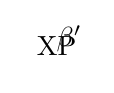
\begin{tikzpicture}[baseline=(root.base)]
        \Tree [.\node(root){XP}; [.$\beta$ ] [.XP [.X ] [.YP [.Y ] [.ZP [.WP [.QP [.Q ] ] [.W ] ] [.Z$'$ [.Z ] ] ] ] ] ]
    \end{tikzpicture}
\z

\noindent The initial \gls{RPM}\is{reduced phrase marker} is \eqref{ex:33.10}:

\ea\label{ex:33.10}$\{\text{XP, X YP, X Y ZP, X Y WP Z, X Y QP W Z, X Y Q W Z$'$, X Y Q Z}\}$
\z

\noindent And the derived \gls{RPM}\is{reduced phrase marker} is \eqref{ex:33.11}:

\ea\label{ex:33.11}$\{$XP, $\beta$ XP, $\beta$ X YP, $\beta$ X Y ZP, $\beta$ X Y WP Z, $\beta$ X Y QP W Z, $\beta$ X Y Q W Z$'$, \\$\beta$ X Y Q W Z$\}$
\z

Once again, the initial set is not a subset of the derived set. In fact, as
with the LSLT \glspl{PM}, there is no obvious simple
set-theoretic relation at all between them.

This is a special case of a more pervasive limitation of such purely
set-theoretic formalizations: constituents are never sub-structures (subsets in
this instance), nor are many core syntactic configurations, such as the
template for a specifier.

Surprisingly, attaching at the very \enquote{bottom} does yield a superset of the
initial set, the exact opposite of the evidently desired result. We illustrate
this beginning with the simple structure in \eqref{ex:33.2}, repeated here, followed by the
\gls{RPM} (which, as noted earlier, is identical to the
LSLT \gls{PM}\is{phrase marker} in this case):

\ea\label{ex:33.12}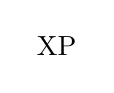
\begin{tikzpicture}[baseline=(root.base)]
    \Tree [.\node(root){XP}; [.X ] [.YP [.Y ] [.ZP [.Z ] ] ] ]
\end{tikzpicture}
\z

\ea\label{ex:33.13}$\{\text{XP, X YP, X Y ZP, X Y Z}\}$
\z

\noindent This time, adjoin $\beta$ at the bottom, in extreme violation of \gls{EC}:

\ea\label{ex:33.14}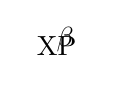
\begin{tikzpicture}[baseline=(root.base)]
        \Tree [.\node(root){XP}; [.X ] [.YP [.Y ] [.ZP [.Z [.$\beta$ ] [.Z ] ] ] ] ]
    \end{tikzpicture}
\z

\noindent The new set is \eqref{ex:33.15}:

\ea\label{ex:33.15} $\{\text{XP, X YP, X Y ZP, X Y Z, X Y $\beta$ Z}\}$
\z

But surprisingly this time the original object is not tampered with as
\eqref{ex:33.13} $\subset$ \eqref{ex:33.15}. It is safe to conclude,
then, that if Chomsky's deduction of \gls{EC}\is{extension condition} is to be maintained, neither
classic set-theoretic formalization of \isi{phrase structure} is appropriate.

In summary, while producing the \enquote{wrong} result, \glspl{RPM} have a
well-defined notion of substructure. For example, $\eqref{ex:33.13}\subset
\eqref{ex:33.15}$ is a subset relation, and the defining relations of an
\gls{RPM} -- precedence and dominance -- are \enquote{preserved} by this
inclusion (for example, the monostring X YP dominates the monostring X Y ZP in
\eqref{ex:33.13}, as does the corresponding monostring in
\eqref{ex:33.15}).

There is also a clear notion of \emph{isomorphism} between R\glspl{PM}, which
will be important in \sectref{sec:33.3.2}. Roughly, if $N$ and $M$ are two sets of nonterminals
and $T$ and $S$ sets of terminals, a pair of bijections $f: N\rightarrow M$ and
$g:T\rightarrow S$ extends to a bijection between sets of strings $(f+g)^*:
(N\cup T)^*\rightarrow (M\cup S)^*$ (replacing each nonterminal symbol $A$ in a
string from $(N\cup T)^*$ with $f(A)$ and each terminal symbol $t$ with
$g(t)$) and hence between monostrings. Given such bijections, we can compare
R\glspl{PM} $F$ and $G$ consisting of monostrings from $(N\cup T)^*$ and
$(M\cup S)^*$, respectively, by using the bijection $(f+g)^*$ restricted to
$F\subset(N\cup T)^*$ and $G\subset (M\cup S)^*$ (if possible). We could say
that two \glspl{RPM} $F$ and $G$ over $(N,T)$  and $(M,S)$ respectively are
isomorphic if we can rename monostrings from $F$ as monostrings in $G$ along
the bijection, and vice-versa (using the inverse of $(f+g)^*$ restricted to
$G\rightarrow F$), extending to a bijection $F\cong G$, such that two
monostrings $\phi$ and $\psi$ in $F$ are in a precedence or dominance relation
exactly when the corresponding monostrings in $G$ are.

%\subsection{Extensive operations}

Before proceeding, we note in passing that it is not only the case that in the
LSLT model, attachment at the top does not ``preserve
structure'', but also that attachment at the top is literally impossible, at
least for a transformation.  Transformations in that framework consist of a
\gls{SA} and a \gls{SC2} (\glsdesc{SC2}). The former determines whether the T
is applicable to a particular \gls{PM}\is{phrase marker}, while the latter
indicates the operation to be performed.  An \gls{SA} is a sequence of
``terms'', each term a (string) variable, a constant (i.e., a syntactic
symbol), or a linear combination of any of the preceding.  Consider Chomsky's
auxiliary transformation ``affix hopping'' as presented by
\textcite{Chomsky1957}. The following is one of a family of 20 \glspl{SA}
embodied by the T:\largerpage[2]

\ea\label{ex:33.16}X -- \emph{past} -- V -- Y
\z

Applicability is determined by comparing the \gls{SA} with the members of the
set to establish satisfaction. Any string satisfies a variable, while a
constant is satisfied only by that very symbol. The T with \gls{SA} in
\eqref{ex:33.16} is applicable to the \gls{PM}\is{phrase marker} pictorially represented in
\eqref{ex:33.17}.

\ea\label{ex:33.17}\begin{tikzpicture}[baseline=(root.base)]
    \Tree [.\node(root){S}; [.NP [.NP\tss{sing} [.John ] ] ] [.VP [.Verb [.Aux [.C [.past ] ] ] [.V [.walk ] ] ] ] ]
\end{tikzpicture}
\z

\noindent The \gls{PM}\is{phrase marker} is in \eqref{ex:33.18}.

\ea\small\label{ex:33.18}$\{$S, NP VP, NP Verb, NP Aux V, NP Aux walk, NP C V, NP C walk, NP past V, NP past walk, NP\tss{sing} VP, NP\tss{sing} Verb, NP\tss{sing} Aux V, NP\tss{sing} Aux walk, NP\tss{sing} C V, NP\tss{sing} C walk, NP\tss{sing} past V, NP\tss{sing} past walk, John VP, John Verb, John Aux V, John Aux walk, John C V, John C walk, John past V, John past walk$\}$
\z

In this case, applicability of the transformation is established by any of 3
members of the set:

\ea\label{ex:33.19}NP past V\hspace{5mm} NP\tss{sing} past V\hspace{5mm} John past V
\z

Notice that every member of any \gls{PM}\is{phrase marker} has symbols in a linear order; every
pair of symbols in a member are in the precedence relation. Thus, the symbols
in any \gls{SA} are likewise necessarily in a linear order. Thus, a symbol can
adjoin to one that follows it (as in affix hopping, where past will adjoin to
V), or to one that precedes it. The result of the operation is in
\eqref{ex:33.20}.\largerpage[2]

\ea\label{ex:33.20}\begin{tikzpicture}[baseline=(root.base)]
        \Tree [.\node(root){S}; [.NP [.NP\tss{sing} [.John ] ] ]
[.VP [.Verb [.Aux [.C ] ] [.V [.V [.walk ] ] [.past ] ] ] ] ]
\end{tikzpicture}
\z

An operation that would adjoin a symbol to a dominating symbol is literally
unstatable. But any singulary \isi{movement} T satisfying the \glsdesc{EC} would have
to do exactly this. Suppose, for example, we wanted to apply a C fronting type
operation (something like Chomsky's T$_\text{q}$) to \eqref{ex:33.17}, but
which would left-adjoin C to S (in accord with \gls{EC}), as pictured in
\eqref{ex:33.21}:

\ea\label{ex:33.21}\begin{tikzpicture}[baseline=(root.base)]
    \Tree [.\node(root){S}; [.C [.past ] ] [.S [.NP [.NP\tss{sing} [.John ] ] ] [.VP [.Verb [.Aux ] [.V [.walk ] ] ] ] ] ]
    \end{tikzpicture}
\z

In the LSLT formalism C and S would both have to be
mentioned in the \gls{SA}. So perhaps the \gls{SA} could be
(\ref{ex:33.22}a) or (\ref{ex:33.22}b):

\ea\label{ex:33.22}
    \ea X--S--C--Y
    \ex X--C--S--Y
    \z
\z

But now look again at the \gls{PM}\is{phrase marker} \eqref{ex:33.18} to
which we would want to apply \eqref{ex:33.22}.  There is no member of that
set that contains both S and C, so the transformation could never apply. This
example is completely representative. No \isi{movement} transformation in the
LSLT framework would ever be able to apply in accord with
\gls{EC}.\footnote{As a reviewer observes, older formulations of the cyclic
    constraint, as in \citet{Chomsky1965} or the strict cycle condition of
\citet{Chomsky1973}, do not run into this difficulty, since they only required
operations to target topmost domains, and not the root per se.}

Interestingly, the L\&K framework also forbids EC-satisfying operations, but
only by stipulation. Within that model, as noted above, the phrase markers\is{phrase marker} are
R\glspl{PM}, sets consisting of the terminal string and monostrings.
Determination of transformational applicability then has to be somewhat
different. In particular, it is small sets of monostrings, rather than single
ones, that are relevant. L\&K provide a definition of precedence between
monostrings, and then simply stipulate in their definition of ``basic
analyzability'' that any qualifying set of monostrings must be pairwise in the
precedence relation. That line of their definition can be eliminated leaving
the remainder intact. The effect of this simplification would be to allow a set
of monostrings not in the precedence relation, and hence in the dominance
relation, to qualify. And this, of course, would allow EC-satisfying
operations.

\section{Bare phrase structure}

Bare phrase structure (\glsunset{BPS}\gls{BPS}, \citealt{ColSta2016}
(C\&S); \citealt{Chomsky2000,fukui2011merge}) takes an
alternative approach to phrase-markers. \gls{BPS}\is{bare phrase structure} uses the set-theoretic
$\in$-relation to describe constituency. We fix the instantiation of \gls{BPS}
described in \citet{Chomsky2000,Chomsky2008} and formalized in
C\&S.

In these models, \textsc{merge} is a structure-building operations which takes
two objects $A$ and $B$ and forms $\{A,B\}$.\footnote{C\&S,
Def.\ 13.} From this definition, we can recover an ``immediately contains''
relation between the objects $A$ and $B$ and $\{A,B\}$ by using the elementhood
relation.  Explicitly, we say that $X$ is \emph{immediately contained} in $Y$
if and only if $X\in Y$.\footnote{C\&S, Def.\ 8.} General
\emph{containment} is defined as the transitive closure of this relation.
Explicitly, we can inductively define containment by saying that $X$ is
contained in $Y$ if $X\in Y$ or $X\in Z$ for some $Z$ contained in $Y$.

Strictly speaking, this is a relation which is defined on the entire model of
the ambient set theory, not on a single set $X$ which represents a single
syntactic object, as in the case of the precedence and dominance relations
between elements of an \gls{RPM}\is{reduced phrase marker}. That is,
containment is a relation between sets in the entire class of sets, not between
elements (``nodes'') of a single syntactic object. Accordingly, a substructure
with respect to the $\in$ relation refers not to a subset of any object in the
model, but rather to a \emph{submodel} of the model of set
theory.\footnote{\citet{chang1990model}.}

It is straightforward to show that constituents are not in general subsets of a
\gls{BPS} syntactic object $X$.

\ea\label{ex:33.23}Let $A$, $B$, $C$, and $D$ be lexical items or complex
syntactic objects.\\
    Construct
    $X=\textsc{merge}(A,\textsc{merge}(B,\textsc{merge}(C,D)))=\{A,\{B,\{C,D\}\}\}$.
    Then, $\{C,D\}$ is contained in $X$, but $\{C,D\}\not\subset X$.
\z

As syntactic objects $X$ are also not models of set theory, but rather the
elements of such a model, the submodel relationship which preserves the $\in$
relation also cannot be the correct notion of substructure for syntactic
objects.

We now present arguments that the $\in$ relation, and its transitive closure,
while providing an accurate characterization of the \emph{containment}
relation,\footnote{Ignoring issues relating to \enquote{occurrences} of lexical
items -- i.e. non-tree structures resulting from the elementhood graphs of
sets.} do not pro\-vide a \emph{substructure} relation between syntactic
objects.  Unfortunately, constituency cannot be used to determine the
appropriate notion of substructure, since, in trees, \enquote{$A$ contains $B$}
is coextensive with ``the constituent dominated by $B$ is a substructure of the
constituent dominated by $A$''. In other words, we cannot tell the containment
relation apart from substructure inclusions between constituents. However, in
slightly relaxed notions of substructures, $\in$ is clearly behaving as a
primitive containment relation between nodes, and not a substructure inclusion.
We turn to some motivating examples.

In C\&S, lexical items are treated as a triple of sets of
features (\textsc{sem}, \textsc{syn}, and \textsc{phon}).  The features of a
syntactic object $X$ are formalized externally with a \textsc{triggers}
function. C\&S keep track of which features have been
satisfied by removing elements from the sets of features associated to $X$ via
\textsc{trigger}. Chomsky suggests in \emph{Categories and transformations} (CT,
\citeyear[Chapter 4]{Chomsky1995}) that
certain formal features may be \emph{erased} upon satisfaction, or at the
interfaces.\footnote{\citet[280]{Chomsky1995}: \enquote{Erasure is a `stronger
form' of deletion, eliminating the element entirely so that it is inaccessible
to any operation, not just to interpretability at \gls{LF}.}} We first look at how
C\&S formalize their calculus of features.
C\&S's feature calculus is meant to capture this intuition.

\ea\label{ex:33.24}(C\&S Def.\ 26) \textsc{triggers} is any
function from each syntactic object $A$ to a subset of the trigger features of
A, meeting the following conditions:
    \begin{xlisti}
        \ex   If $A$ is a lexical item with $n$ trigger features, then
        \textsc{triggers}($A$) returns all of those $n$ trigger features. (So when
        $n=0$, \textsc{triggers}($A)=\{\}$.)
    %    \exi{(ii)}  If $A$ is a lexical item with $n$ trigger features, then
    %    \textsc{triggers}($A$) returns all of those $n$ trigger features. (So when
    %    $n=0$, \textsc{triggers}($A)=\{\}$.)
        \ex If $A$ is a set, then $A=\{B,C\}$ where \textsc{triggers}($B$)
        is nonempty, and \textsc{triggers}($C)=\{\}$, and
        \textsc{triggers}($A)=\textsc{triggers}(B)-\{\text{TF}\}$, for some trigger
        feature TF $\in \textsc{triggers}(B)$.  Otherwise, \textsc{triggers}($A$)
        is undefined.
        \ex Otherwise, \textsc{triggers}($A$) is undefined.
    \end{xlisti}
\z

This goes hand in hand with their definition of triggered merge\is{Merge}.

\ea\label{ex:33.22b}(C\&S Def.\ 27) Given any syntactic
objects $A$, $B$, where \textsc{triggers}($A)\neq \{\}$ and
\textsc{triggers}($B)=\{\}$, \textsc{merge}$(A,B)=\{A,B\}$.  \z

The idea is that two items may only merge\is{Merge} when one has remaining trigger
features, and the other does not. If defined, the trigger features of $\{A,B\}$
are just those of the triggering object $A$ with the triggering feature
removed. Notice, however, that \textsc{trigger} keeps track of the feature
changes externally, in that no features of heads contained in $A$ or $B$ are
changed. Under such a method, the set-theoretic structure of syntactic objects
alone does not encode the featural changes. We want to \enquote{internalize} the
feature calculus so that \textsc{merge} actually results in changes in the
structure of the objects it combines.

We have at least two reasonable options for formally realizing these notions of
erasure/deletion within a syntactic object itself: by removing the element in
question from the syntactic object, or by changing the element in some way
which marks it as inoperative. We will show that either method results in an
object which the $\in$ relation and its transitive closure both fail to treat
as related to the original object in any straightforward way. We will extend
the argument to cases of \textsc{agree}.

\subsection{Method one: Removal of the feature}

For any sets $A$ and $B$, we can construct a set $A-B=\{a\in A:a\not\in B\}$,
their \emph{difference}, which removes $B$-elements from $A$.

Let $A$ be a lexical item and $X$ and $Y$ be syntactic objects (lexical items
or otherwise). We treat lexical items as in CT, where $A$ is literally a
\emph{set} of features. Take the syntactic object
$\textsc{merge}(A,Y)=\{A,Y\}$.\footnote{For simplicity, we delete no features
in the first step, though the argument still holds if we do remove a feature of
$A$ (or $Y$) during this first step.} Suppose that when this object is merged
with $X$, a feature of the head $A$ is checked, removing $f\in A$, resulting in
the object $\{X,\{A-\{f\},Y\}\}$. Alternatively, if features are not deleted in
syntax, we may say that some interface only sees the structure
$\{X,\{A-\{f\},Y\}\}$, which should be a substructure of $\{X,\{A,Y\}\}$.

In the first case, we should like to describe in what sense $\{A-\{f\},Y\}$ is
a substructure of $\{A,Y\}$ in that they have the same \isi{phrase structure},
with the former simply missing a feature of the latter, so that we can state a
form of the \gls{EC}\is{extension condition}. In the second case, we should
like to describe how $\{X,\{A-\{f\},Y\}\}$ is a substructure of
$\{X,\{A,Y\}\}$.

As expected, a subset relation fails to hold in both cases:
$\{X,\{A-\{f\},Y\}\}\not\subset\{X,\{A,Y\}\}$, and
$\{A-\{f\},Y\}\not\subset\{A,Y\}$. However, there is also no containment
relation between the syntactic objects. In fact, there is no straightforward
set-theoretic relation between these objects. While a subset relation
$\{A-\{f\}\subset A\}$ does hold, $\{A-\{f\},Y\}\not\subset\{A,Y\}$. More
generally, for any constituent $M$ containing a head $A$ from which we remove a
feature, the resulting constituent $M'$ will simply be a distinct set
from $M$ (often with the same number of elements as $M$). In this example,
$\{X,\{A-\{f\},Y\}\}$ and $\{X,\{A,Y\}\}$ have the same number of elements,
though $A$ and $A-\{f\}$ do not, assuming $A$ is finite.

On the other hand, there are canonical ways to draw graph-theoretic objects
from well-founded sets. One method produces trees: draw a set $X$ as a root,
and write all of its elements as immediate daughters. We repeat the process at
each child, writing the same element multiple times if necessary. This process
is described in \citet{aczel}.

\ea\label{ex:aczel}
    \hspace*{-.75cm}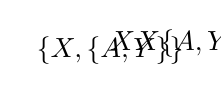
\begin{tikzpicture}[baseline=(root.base)]
    \Tree   [.\node(root){$\{X,\{A,Y\}\}$};
                [.$X$ \edge [roof]; {elements contained in $X$} ]
                [.$\{A,Y\}$
                    [.$A$
                        [.$a_1$ ]
                        [.$\ldots$ ]
                        [.$f$ ]
                        [.$\ldots$ ]
                        [.$a_n$ ]
                    ]
                    [.$Y$ \edge [roof]; {elements contained in $Y$} ]
                ]
            ]
    \end{tikzpicture}
\z

A \emph{graph} can be defined as a set $X$ together with a relation $R\subset
X\times X$. For syntactic objects $K$, we can define a set $X$ of occurrences
of contained elements, with $R\subset X\times X$ being the immediate
containment relation between the appropriate occurrences; see
C\&S (\S 4, Def.\ 18) for a formal treatment.

We can define a \emph{subgraph} relation between two graphs $(X,R)$ and $(Y,S)$
if $X\subset Y$ and we have a relation $xRx'$ for $x,x'\in X$ if
and only if $xSx'$ in $Y$. We can then form the graph-theoretic tree
associated to $\{X,\{A-\{f\},Y\}\}$, which is clearly a subgraph of the graph
in \REF{ex:aczel}. We could similarly use the containment relation in
place of the immediate containment relation, which would describe the syntactic
objects as partially ordered sets, with the substructure relation being a
subspace inclusion of finite partial orders.

\subsection{Method two: Changing (the value of) a feature}\label{sec:33.3.2}

Changing the \enquote{value} or otherwise adding diacritical marks to an element is
another way to formally represent the status of a feature in a syntactic
object.

In this case, suppose that we have again constructed $\{A,Y\}$ which we intend
to merge\is{Merge} with $X$ in a way which will alter a feature $f\in A$. This
alteration could be realized as a bijection $m:A\rightarrow A'$, where $A'$ is
the same set as $A$, except the feature $f$ has been replaced by
$\overline{f}$, the ``inoperative'' form of $f$.

However, $\{A,Y\}$ is not a subset of $\{X,\{A',Y\}\}$, nor do we have a
containment relation between the two sets. Much like subsets are not the
relevant notion of substructure for \gls{BPS}\is{bare phrase structure} sets, neither will bijection be
the appropriate notion of isomorphism. For, depending on whether we allow
\textsc{merge} to combine identical sets or not, every \gls{BPS}\is{bare phrase structure} set will have
cardinality 1 or 2, and hence be in a bijection with the set $1=\{0\}$ or
$2=\{0,1\}$. So while $\{A',Y\}$ and $\{A,Y\}$ are \enquote{isomorphic} in that there
is a bijection between them, so are they both isomorphic to $\{X,\{A,Y\}\}$,
showing that this is not the correct notion of \enquote{isomorphism} between the
objects, in that it totally ignores constituency.

Again, we may convert $\{A,Y\}$ and $\{X,\{A',Y\}\}$ into graph- or
order-theoretic trees. We can define an isomorphism between graphs $(X,R)$ and
$(Y,S)$ as a bijection $m:X\rightarrow Y$ such that $xRx'$ in $X$ if and only
if $(mx) S (mx')$ in $Y$ (or similarly, an isomorphism of partial orders as a
bijection $m:P\rightarrow Q$ such that $x\leq x'$ in $P$ if and only if
$m(x)\preceq m(x')$ in $Q$). Using these definitions, two graph- or
order-theoretic trees $(X,R)$ and $(Y,S)$ will be isomorphic if and only if
they have the same number of nodes with the same constituency
relations.\footnote{Though, this ignores the \enquote{occurrence} relations which
    indicate which nodes are \enquote{copies} of others. On the other hand, the
multidominant picture of a tree, called the \emph{canonical picture} in
\citet{aczel}, and given in Fig. 3 in C\&S, would not have
this issue, and could be used instead.} Using this definition, the graphs
associated to $\{A,Y\}$ and $\{A',Y\}$ will be isomorphic, such that $\{A,Y\}$
is isomorphic to a subgraph of $\{X,\{A',Y\}\}$ in the appropriate way.

Alternatively, we might think of this \enquote{value} or \enquote{activity} as a property of a
feature which is explicitly part of its structure. This again has a
straightforward formalization when the syntactic objects are graphs: we define
a graph-with-value as a graph $(X,R)$ together with a function
$\nu:X\rightarrow\{\top,\bot\}$ where we interpret $\nu (x)=\top$ as meaning
``$x$ is inactive''. We define a homomorphism between graphs-with-values
$f:(X,R,\nu)\rightarrow (X',R',\nu')$ as a graph homomorphism such that if
$\nu(x)=\top$, then $\nu'(f(x))=\top$, i.e. inactive features stay inactive,
but active features may be deactivated. Using this structure, the inclusion of
an operand $A$ into larger object $X$, while deactivating a feature in $A$,
would be a homomorphism.

\subsection{Agree}

The above examples showed that the feature-deletion and feature-valuation\linebreak
methods of modeling \textsc{merge} do not lead to substructure embeddings or
homomorphisms between \gls{BPS}\is{bare phrase structure} sets in any obvious sense.  In contrast,
relations between derived syntactic objects are straightforward when
represented as graphs (possibly with extra structure).
\citet{chomsky1999derivation} has a \enquote{valuation} version of \isi{agreement}, which is
subject to similar analysis as the valuation case for selection above. We look
now at a feature-sharing approach to \isi{agreement}, and similarly show that the
structural relation between the input structures and output structures is given
straightforwardly by graph homomorphisms, while there is no clear associated
notion for sets.

\citet{frampton2000agreement} give an explicit architecture for \isi{agreement} as
feature-sharing using the set-theoretic structure of \gls{BPS}\is{bare phrase structure}:

\blockquote[{\citealt{frampton2000agreement}}]{Consider [\eqref{ex:33.25}]
    and suppose that \isi{Agree} applies to the pair of nodes.

{\small
\ea\label{ex:33.25}$\{$Num${}_1$, Case${}_2$, \ldots$\}$,
$\{$Per${}_3$, Num${}_4$, Case${}_5$,\dots$\}$
\z}

[\ldots] suppose that \isi{Agree} induces feature sharing, so that matching features
coalesce into a single shared feature, which is valued if either of the
coalescing features is valued. So [\eqref{ex:33.25}] produces:

{\small
\ea\label{ex:33.26}$\{$Num${}_6$, Case${}_7$, \ldots$\}$,
$\{$Per${}_3$, Num${}_6$, Case${}_7$,\dots$\}$
\z}

The value of Num$_6$ is the coalescence of the values of Num$_1$ and Num$_4$.
The value of Case$_7$ is the coalescence of the values of Case$_2$ and
Case$_5$. New indices were chosen, but index 6, for example, could just as well
have been 1 or 4. The choice of index is not a substantive question, assuming
that it is suitably distinguished.

If the two coalescing features are both valued to start with, it is not clear
that the result is coherent. But this will never arise, because \isi{Agree} is driven
by an unvalued feature. A picture will make the idea clearer. \isi{Agree} takes
[(\ref{ex:33.27}a)] into [(\ref{ex:33.27}b)], assuming that none of the
features indicated by the \isi{ellipsis} marks match.

\ea\label{ex:33.27} a.\hspace{6.25cm}b.
    \begin{tikzpicture}[baseline=(a.base), font=\smaller, sibling distance=-2pt]

        \Tree 	[.\node(a){A};
                    {\makebox[0pt][l]{Num}\phantom{Case}\\{}[]}
                    {Case\\{}[]}
                    {\makebox[0pt][r]{\dots}\phantom{Case}\\{}[]}
                ]

        \begin{scope}[xshift=2.75cm]

        \Tree   [.\node(b){B};
                    {Per\\{}[\Third]}
                    {Num\\{}[\Pl]}
                    {Case\\{}[]}
                    \dots{}
                ]

        \end{scope}

        \begin{scope}[xshift=6.0cm]

        \Tree [.\node(a2){A}; \dots{} ]

        \end{scope}

        \begin{scope}[xshift=8.0cm]

        \Tree   [.\node(c){B};
                    {Per\\{}[\Third]}
                    \node(num){Num\\{}[\Pl]};
                    \node(case){Case\\{}[]};
                    \dots{}
                ]

        \end{scope}

        \draw (a2.south) to (num.north);
        \draw (a2.south) to (case.north);

        \node [below left=.5cm of a2, align=center, font=\smaller]
            {Agree\\$\longrightarrow$};

    \end{tikzpicture}
\z}

The arrow \enquote{Agree} in Frampton \& Gutmann's figure can clearly be viewed
as a pair of graph homomorphisms from each graph on the lefthand side to the
graph on the righthand side, or as single graph homomorphism from the
``structured disjoint union''\footnote{Formally, this is the \emph{coproduct}
    of graphs in the category of directed graphs.} of the graphs on the
    lefthand side to the graph on the righthand side. If we view the valuations
    as properties attached to the nodes of the graph, then we can additionally
    view this map \isi{Agree} as a graph homomorphism which preserves those
    properties (e.g.\ a \Pl{} node gets taken to a \Pl{} node).

However, it is again difficult to describe the relationship above when we view
the objects as \gls{BPS}\is{bare phrase structure} sets. Usually at least one of $A$ or $B$ above will be
in a phrase when \isi{agreement} is applied. Suppose it is $B$, and we have
$B\in\ldots\in X$. We intend to construct from $A$ and $X$ an object
$\{A',X'\}$, where $A'$ and $X'$ are exactly $A$ and $X$, but where the number
and case features\is{case!case features} have been replaced accordingly. Again, we will have no
subset, containment, or other obvious set-theoretic relation between $A$ or $X$
and $\{A',X'\}$.

Another application of isomorphism\is{isomorphism} appears implicitly here.
\citeauthor{frampton2000agreement} note that the specific index for the element
representing the shared feature does not matter, so long as it is suitably
distinguished. Again, while the set-theoretic statement of this is somewhat
complex (and relies on knowing the specific indices used elsewhere in syntactic
objects contained in the current one), the graph-theoretic notion is quite
elegant: the righthand side above is determined up to isomorphism of graphs
(possibly with values assigned to nodes).

\section{The extension condition in the theory of phrase structure}

Using LSLT phrase markers\is{phrase marker}, constituents
do not arise as substructures in any straightforward way. Accordingly, even if
we allow operations which have the effect of the \gls{EC}\is{extension
condition}, it will not be strictly true that the inputs to the operation are
substructures of the output.

In \gls{BPS}\is{bare phrase structure}, if we represent feature-changes at all
in syntactic objects, either by means of deletion or alteration, it is no
longer straightforward in what sense the inputs to \textsc{merge} are
substructures of or are contained in the output.  C\&S and
\citet{Chomsky2000} only avoid this problem by not annotating the
\enquote{feature-updates} in the syntactic objects themselves, the former by
keeping track of the features in \enquote{scoreboard} sets external to the
syntactic object (though relevant to determining properties of it, such as
labeling), where the latter does not address the treatment of features in
syntactic objects formally at all.

If we choose the second method which \enquote{alters} features, and implement it in
the syntax, then the input $\{A,Y\}$ to \textsc{merge} will not be a
substructure of the output $\{X,\{A',X\}\}$ or immediately contained in it.
Similarly, no substructure of $\{A,Y\}$ will be contained in
$\{X,\{A-\{f\},Y\}\}$ if the first method is used in syntax. Both lead to
complications in stating the extension condition for \gls{BPS}\is{bare phrase structure}.

However, \gls{BPS}\is{bare phrase structure} sets can be viewed as an \enquote{encoding} of graphs or partial
orders using some canonical translation of them. These graphs essentially arise
from constructing a set of elements contained in a syntactic object $X$
(possibly with occurrences), and restricting the $\in$ relation between sets to
this set.  In C\&S, many of the important structural
properties of syntactic objects -- e.g.\ c-command, relative minimality and
maximality (of projections), and specifiers -- are similarly defined not on a
syntactic object $X$ itself but the associated graph of occurrences of elements
contained in $X$, using a relation based on $\in$ as its ``edge relation''.
Accordingly, the graph- and order-theoretic representation of \gls{BPS}\is{bare
phrase structure} objects provides a coherent notion of substructure and
isomorphism, which makes statement of the \gls{EC}\is{extension condition}
straightforward using either method described above.

Pure set-theoretic representations limit the distinctions that can be made. To
the extent that human language does not rely on the encoding of the
mathematically unavailable distinctions, we should favor a theory based on such
representations, as we want to limit the descriptive power of the theory as
much as is empirically possible, in line with the general Chomskian program.
But where we do need to make such distinctions in a full account of human
language, we must move to a richer theory of representations, as we have
explored here. Studying substructures and isomorphism\is{isomorphism} as they can be used to
state the \gls{EC}\is{extension condition} provide just one example of how understanding formal properties of
the representation of syntactic objects can clarify the relationship between
structure-building operations and the properties of the syntactic objects
themselves.

\printchapterglossary{}

\section*{Acknowledgements}

We are very pleased to help honor Ian Roberts, who has encouraged the field to
rethink so many topics in syntax. We are indebted to the two reviewers, whose
comments helped us substantially improve the presentation.

{\sloppy\printbibliography[heading=subbibliography,notkeyword=this]}
\end{document}
